\documentclass{mwart}
\usepackage{polski}
\usepackage[polish]{babel}
\usepackage{amsfonts}
\usepackage{indentfirst}
\usepackage[utf8]{inputenc}
\usepackage{amsthm}
\usepackage{multirow}
\usepackage{amsmath}
\newtheorem{tw}{Twierdzenie}
\newtheorem{df}{Definicja}
\newtheorem{zd}{Zadanie}
\newtheorem{zdt}[zd]{Zadanie*}
\title{Procesy stochastyczne\\ Zestaw zadań nr 1}
\usepackage{Sweave}
\begin{document}
\Sconcordance{concordance:Zestaw1_PS_2020.tex:Zestaw1_PS_2020.Rnw:%
1 14 1 1 0 2 1 1 6 33 1 1 3 1 2 29 1 1 7 1 5 1 2 6 1}

\maketitle
\begin{zd}
Dana jest funkcja
\begin{displaymath}
F(x) = 0\cdot\pmb{1}_{x\leq 0} + (ax^2+bx)\cdot\pmb{1}_{0<x\leq 1} + 1\cdot \pmb{1}_{x\geq 1}.
\end{displaymath}
Znajdź wszystkie pary liczb $a, b$ dla których funkcja ta jest dystrybuantą. Dla jakich wartości dystrybuanta ta jest ciągła?
\end{zd}

\begin{zd}
Dodatnia liczba naturalna $I$ jest losowana zgodnie z rozkładem $\mathbb{P}(I =n) = \left(\frac{1}{2}\right)^n, n = 1,2, \dots$. Jeśli liczba $I$ przyjmie wartość $n$, wtedy rzucana jest moneta z prawdopodobieństwem wyrzucenia orła równym $e^{-n}$. Znajdź prawdopodobieństwo, że otrzymano orła.
\end{zd}

\begin{zd}
Niech $X_1, X_2, \dots, X_n$ będą niezależnymi zmiennymi losowymi o tym samym rozkładzie z gęstością $f$ i dystrybuntą $F$. Niech $T_k$ będzie k-tą najmniejszą obserwacją. Znajdź rozkład $T_k$ i wektora $(T_1, T_2, \dots, T_n)$.
\end{zd}

%f(1/x)/x^2
\begin{zd}
Niech $X$ będzie zmienną losową przyjmującą dodatnie wartości oraz o gęstości $f$. Znajdź postać gęstości zmiennej losowej $X^{-1}$.
\end{zd}
%5.7.2, 5.7.4
\begin{zd}
Niech $X$ będzie zmienną losową przyjmująca nieujemne wartości i niech $\phi$ będzie rosnącą i różniczkowalną funkcją taką, że $\phi(0) =0$. Udowodnij
\begin{enumerate}
\item $\mathbb{E}X = \int_0^{+\infty}\mathbb{P}(X\geq t)dt$
\item $\sum_{i=1}^{+infty}\mathbb{P}(X \geq n) \leq \mathbb{E}X \leq 1 +\sum_{i=1}^{+infty}\mathbb{P}(X \geq n$ (jaki stąd wniosek na temat całkowalności $X$?)
\item  $\mathbb{E}\phi(X) = \int_0^{+\infty}\phi'(t)\mathbb{P}(X\geq t)dt$
\end{enumerate}
\end{zd}

\begin{zd}
Niech $X, Y$ będą niezależnymi zmiennymi losowym o jednosatjnym rozkładzie na odcinku $(0,1)$. Udowodnij, że zmienne $U = \sqrt{-2\log X}\cos(2\pi Y)$, $V = \sqrt{-2\log X}\sin (2\pi Y)$ są niezależne i mają standardowy rozkład normalny. Czy widzisz jakieś zastosowanie tego twierdzenia?
\end{zd}

%5.10.5
\begin{zd}
Rozkład Cauchy'ego ma następującą gęstość
\begin{displaymath}
c_u(x) = \frac{1}{\pi}\frac{1}{u^2 + x^2}, x\in \mathbb{R}, u >0.
\end{displaymath}
\begin{enumerate}
\item Znajdź wartość oczekiwaną rozkładu Cauchy'ego.
\item Wykaż, że $c_u\ast c_v = c_{u+v}$.
\item Niech $X_1, X_2, \dots, X_n$ będą niezależnymi zmiennymi losowymi o rozkładzie $c_u$. Wykaż, że $(X_1+X_2+\dots +X_n)/n$ również ma rozkład $c_u$.
\item Niech $X, Y$ będą niezależnymi zmiennymi losowymi o standardowym rozkładzie normalnym. Wykaż, że $X/Y$ ma rozkład $c_1$.
\item Niech $X$ ma rozkład jednostajny na przedziale $(-\pi/2, \pi/2)$. Wykaż, że $\tan X$ ma rozkład Cauch'ego $c_1$.
\end{enumerate}
\begin{figure}
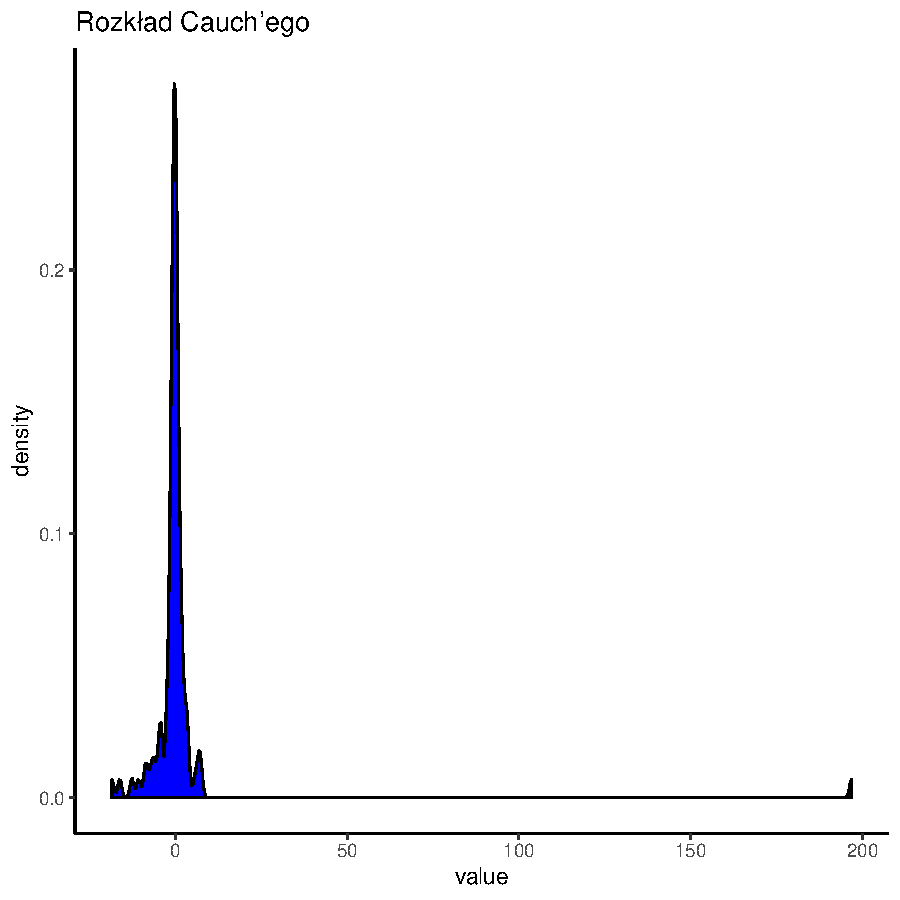
\includegraphics{Zestaw1_PS_2020-002}
\end{figure}
\end{zd}

\begin{zd}
Niech dany będzie wielowymiarowy rozkład normlny z gęstością $g(x,y)=\frac{1}{\sqrt{2}\pi}exp\left(-\frac{x^{2}-2xy+3y^{2}}{2}\right)$. Znajdź parametry tego rozkładu.
\end{zd}

\begin{zd}
Niech $X\sim \mathcal{N}_p\left(\mu, \Sigma \right)$ i niech $A$ będzie macierzą symetryczną. Udowodnij, że
$\mathbb{E}X^TAX = tr(A\Sigma) + \mu^T A \mu$.
\end{zd}

\begin{zd}
Załóżmy, że zmienne losowe $X_1, X_2, \dots, X_{20}$ są niezależne, o jednakowym
rozkładzie $\mathcal{N}(\mu, \sigma^2)$. Niech $Y_5 = X_1 + \dots + X_5$, $Y_{20} = X_1+\dots +X_{20}$. Wyznaczyć warunkową wartość oczekiwaną $\mathbb{E}(Y_5|Y_{20})$.
\end{zd}

\begin{zd}
W grupie studenckiej przeprowadzono test z analizy, w którym można uzyskać od 0 do 100 punktów. Przeciętna liczba punktów uzyskiwanych przez studenta wynosi 40, a odchylenie standardowe 20. Zakładając, że wyniki studentów są niezależnymi zmiennymi losowymi o tym samym rozkładzie prawdopodobieństwa, obliczyć prawdopodobieństwo tego, że średnia liczba punktów w 150 osobowej grupie studenckiej będzie większa od 45.
\end{zd}

\begin{zd}
Załóżmy, że przy składaniu książki w drukarni każda litera ma prawdopodobieństwo 0.0001, że zostanie złożona błędnie. Po złożeniu książki szpalty czyta korektor, który znajduje każdy błąd z prawdopodobieństwem 0.5. Znaleźć prawdopodobieństwo, że w książce o stu tysiącach znaków drukarskich pozostaną po korekcie nie więcej niż dwa błędy.
\end{zd}

%5.9.11
\begin{zdt}
Zbiór Cantora $C$ to zbiór wszystkich liczb $t$ postaci
\begin{displaymath}
t = \frac{t_1}{3} + \frac{t_2}{3^2} + \dots + \frac{t_n}{3^n}+\dots,
\end{displaymath}
gdzie $t_i\in \{0, 2\}$. Zauważmy, że każda liczba ze zbioru $C$ ma jednoznaczną reprezentację. Określmy funkcję schodkową przekształcającą zbiór Cantora na odcinek $[0, 1]$. Dla liczb $t$ ze zbioru $C$ połóżmy
\begin{displaymath}
\phi(t) = \frac{1}{2}\left(\frac{t_1}{2} + \frac{t_2}{2^2} + \dots + \frac{t_n}{2^n}+\dots\right).
\end{displaymath}
Poza zbiorem Cantora kładziemy odpowiednie stałe tak, aby funkcja, o dziedzinie rozszerzonej z $C$ do $[0, 1]$
była niemalejąca.
\begin{enumerate}
\item Wykazać, że jest to dystrybuanta ciągła, ale nie absolutnie ciągła (nie posiada gęstości).
\item Obliczyć wartość oczekiwaną zmiennej o tej dystrybuancie.
\end{enumerate}
\end{zdt}

\begin{zdt}
Udowodnij, że każde $\sigma$-ciało, jeśli jest nieskończone to musi być nieprzeliczalne.
\end{zdt}

\begin{zd}
Od jakiej wartość (ilości sumownaych składników) można powiedzieć, że działa centralne twierdzenie graniczne? Zaprojektuj eksperyment numeryczny, który dla kilku rodzin rozkładów pozwoli ocenić tą wartość.

\begin{figure}
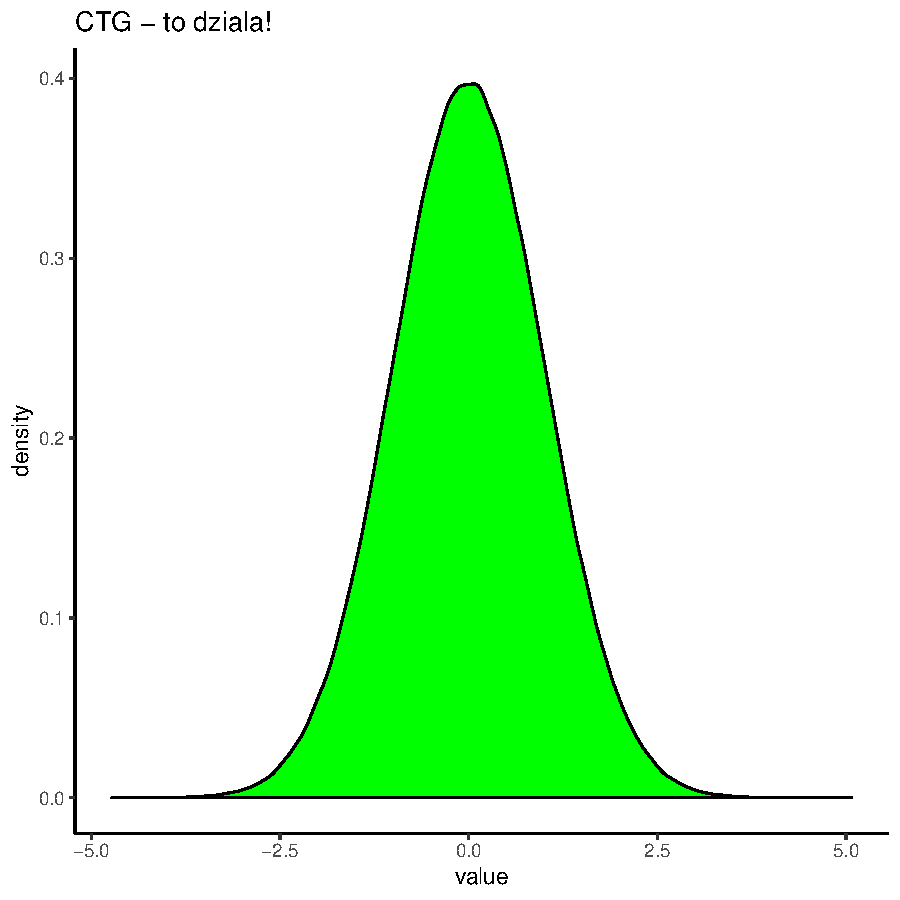
\includegraphics{Zestaw1_PS_2020-004}
\end{figure}
\end{zd}

% \begin{zd}
% Niech $X_1, X_2, \dots$ będzie ciągiem niezależnych zmiennych losowych takich, że $X_n \tilde B(n, p_n)$, gdzie $p_n = \lambda/n$ dla pewnego $\lambda > 0$. Przy pomocy eksperymentu numerycznego zaproponuj rozkład graniczny tego ciągu.
% \end{zd}
\end{document}
